%\VignetteIndexEntry{Introduction to the dataRetrieval package}
%\VignetteDepends{}
%\VignetteSuggests{}
%\VignetteImports{}
%\VignettePackage{}

\documentclass[a4paper,11pt]{article}

\usepackage{amsmath}
\usepackage{times}
\usepackage{hyperref}
\usepackage[numbers, round]{natbib}
\usepackage[american]{babel}
\usepackage{authblk}
\renewcommand\Affilfont{\itshape\small}
\usepackage{Sweave}
\renewcommand{\topfraction}{0.85}
\renewcommand{\textfraction}{0.1}
\usepackage{graphicx}


\textwidth=6.2in
\textheight=8.5in
\parskip=.3cm
\oddsidemargin=.1in
\evensidemargin=.1in
\headheight=-.3in

%------------------------------------------------------------
% newcommand
%------------------------------------------------------------
\newcommand{\scscst}{\scriptscriptstyle}
\newcommand{\scst}{\scriptstyle}
\newcommand{\Robject}[1]{{\texttt{#1}}}
\newcommand{\Rfunction}[1]{{\texttt{#1}}}
\newcommand{\Rclass}[1]{\textit{#1}}
\newcommand{\Rpackage}[1]{\textit{#1}}
\newcommand{\Rexpression}[1]{\texttt{#1}}
\newcommand{\Rmethod}[1]{{\texttt{#1}}}
\newcommand{\Rfunarg}[1]{{\texttt{#1}}}

\begin{document}
\Sconcordance{concordance:dataRetrieval.tex:dataRetrieval.Rnw:%
1 126 1 49 0 1 7 15 1 1 14 55 1 3 0 36 1 2 0 11 1 24 %
0 24 1 3 0 23 1 3 0 6 1 7 0 18 1 3 0 25 1 1 0 17 1 9 %
0 6 1 7 0 21 1 8 0 16 1 2 0 11 1 23 0 21 1 9 0 20 1 3 %
0 6 1 17 0 27 1 6 0 11 1 9 0 15 1 20 0 21 1 4 0 21 1 %
4 0 17 1 7 0 22 1 8 0 19 1 4 0 9 1 4 0 78 1 1 2 9 1 1 %
4 4 1 20 0 44 1 4 0 32 1 4 0 21 1 4 0 21 1 37 0 13 1 %
9 0 95 1 4 0 9 1 12 0 13 1 4 0 14 1 4 0 5 1 4 0 23 1 %
18 0 8 1 4 0 55 1}


%------------------------------------------------------------
\title{Introduction to the dataRetrieval package}
%------------------------------------------------------------
\author[1]{Laura De Cicco}
\author[1]{Robert Hirsch}
\affil[1]{United States Geological Survey}



\maketitle
\tableofcontents

%------------------------------------------------------------
\section{Introduction to dataRetrieval}
%------------------------------------------------------------ 
The dataRetrieval package was created to simplify the process of getting hydrologic data in the R enviornment. It has been specifically designed to work seamlessly with the EGRET package: Exploration and Graphics for RivEr Trends (EGRET). See: \url{https://github.com/USGS-R/EGRET/wiki} for information on EGRET.

There is a plethora of hydrological data available on the web. This package is designed specifically to load United States Geological Survey (USGS) hydrologic data to the R enviornment. This includes daily values, real-time (unit values), site information, and water quality sample data. 

For information on getting started in R, downloading and installing the package, see Appendix 1: Getting Started.


%------------------------------------------------------------
\section{USGS Web Retrieval Examples}
%------------------------------------------------------------ 
In this section, we will run through 5 examples, documenting how to get raw data from the web. This includes historical daily values, real-time current values, water quality data, site information, and measured parameter information. We will use the Choptank River near Greensboro, MD as an example.  The site-ID for this gage station is 01491000. Daily discharge measurements are available as far back as 1948.  Additionally, forms of nitrate have been measured dating back to 1964. The functions/examples in this section are for raw data retrieval.  This may or may not be the easiest data to work with.  In the next section, we will use functions that retrieve and process the data in a dataframe very friendly for R analysis.

%------------------------------------------------------------
\subsection{USGS Web Retrieval Introduction}
%------------------------------------------------------------
The United States Geological Survey organizes their hydrological data in fairly standard structure.  Gage stations are located throughout the United States, each station has a unique ID.  Often (but not always), these ID's are 8 digits.  The first step to finding data is discoving this 8-digit ID. One potential tool for discovering data is Environmental Data Discovery and Transformation (EnDDaT): \url{http://cida.usgs.gov/enddat/}.  Follow the example in the User's Guide to learn how to discover USGS stations and available data from any location in the United States. Essentially, you can create a Project Location on the map, set a bounding box (in miles), then search for USGS Time Series and USGS Water Quality Data. Locations, ID's, available data, and available time periods will load on the map and appropriate tabs.

Once the site-ID is known, the next required input for USGS data retrievals is the 'parameter code'.  This is a 5-digit code that specifies what measured paramater is being requested.  A complete list of possible USGS parameter codes can be found here: 

\url{http://nwis.waterdata.usgs.gov/usa/nwis/pmcodes?radio_pm_search=param_group&pm_group=All+--+include+all+parameter+groups&pm_search=&casrn_search=&srsname_search=&format=html_table&show=parameter_group_nm&show=parameter_nm&show=casrn&show=srsname&show=parameter_units}

Not every station will measure all parameters. The following is a list of commonly measured parameters:

% latex table generated in R 2.15.2 by xtable 1.7-0 package
% Thu Jan 24 10:35:50 2013
\begin{table}[ht]
\begin{center}
\caption{Commonly found USGS Parameter Codes}
\begin{tabular}{rll}
  \hline
 & pCode & shortName \\ 
  \hline
1 & 00060 & Discharge [cfs] \\ 
  2 & 00065 & Gage height [ft] \\ 
  3 & 00010 & Temperature [C] \\ 
  4 & 00045 & Precipitation [in] \\ 
  5 & 00400 & pH \\ 
   \hline
\end{tabular}
\end{center}
\end{table}
For real-time data, the parameter code and site ID will suffice.  The USGS stores historical data as daily values however.  The statistical process used to store the daily data is the final requirement for daily value retrievals.  A 5-digit 'stat code' specifies the requested processing.  A complete list of possible USGS stat codes can be found here:

\url{http://nwis.waterdata.usgs.gov/nwis/help/?read_file=stat&format=table}

The most common stat codes are:
% latex table generated in R 2.15.2 by xtable 1.7-0 package
% Thu Jan 24 10:35:50 2013
\begin{table}[ht]
\begin{center}
\caption{Commonly found USGS Stat Codes}
\begin{tabular}{rll}
  \hline
 & StatCode & shortName \\ 
  \hline
1 & 00001 & Maximum \\ 
  2 & 00002 & Minimum \\ 
  3 & 00003 & Mean \\ 
  4 & 00008 & Median \\ 
   \hline
\end{tabular}
\end{center}
\end{table}

%------------------------------------------------------------
\subsection{USGS Site Information Retrievals}
%------------------------------------------------------------
To obtain all of the available site information, use the getSiteFileData function:
\begin{Schunk}
\begin{Sinput}
> library(dataRetrieval)
> # Using defaults:
> siteNumber <- "01491000" # Site ID for Choptank River near Greensboro, MD
> ChoptankInfo <- getSiteFileData(siteNumber)
\end{Sinput}
\end{Schunk}

The available returned data for these for the USGS sites can be viewed in Appendix 2: getSiteFileData. Pulling out a specific example piece of information, in this case station name can be done as follows:
\begin{Schunk}
\begin{Sinput}
> ChoptankInfo$station.nm
\end{Sinput}
\begin{Soutput}
[1] "CHOPTANK RIVER NEAR GREENSBORO, MD"
\end{Soutput}
\end{Schunk}
Site information is obtained from \url{http://waterservices.usgs.gov/rest/Site-Test-Tool.html}

%------------------------------------------------------------
\subsection{USGS Parameter Information Retrievals}
%------------------------------------------------------------
To obtain all of the available information concerning a measured parameter, use the getParameterInfo function:
\begin{Schunk}
\begin{Sinput}
> # Using defaults:
> parameterCd <- "00618" 
> parameterINFO <- getParameterInfo(parameterCd)
\end{Sinput}
\end{Schunk}

The available data for these parameters can be seen in Appendix 2: getParameterInfo. Pulling out a specific example piece of information, in this case station name can be done as follows:
\begin{Schunk}
\begin{Sinput}
> parameterINFO$parameter_nm
\end{Sinput}
\begin{Soutput}
[1] "Nitrate, water, filtered, milligrams per liter as nitrogen"
\end{Soutput}
\end{Schunk}
Parameter information is obtained from \url{http://nwis.waterdata.usgs.gov/nwis/pmcodes/}



%------------------------------------------------------------
\subsection{USGS Daily Value Retrievals}
%------------------------------------------------------------
To obtain historic daily records of USGS data, use the retrieveNWISData function. The arguments for this function are siteNumber, parameterCd, startDate, endDate, statCd, and a logical (true/false) interactive. There are 2 default argument: statCd defaults to "00003" and interactive defaults to TRUE.  If you want to use the default values, you do not need to list them in the function call. Setting the 'interactive' option to true will walk you through the function. It might make more sense to run large batch collections with the interactive option set to FALSE. 

The dates (start and end) need to be in the format "YYYY-MM-DD".  Setting the start date to "" will indicate to the program to ask for the earliest date, setting the end date to "" will ask for the latest available date.

\begin{Schunk}
\begin{Sinput}
> # Using defaults:
> siteNumber <- "01491000" # Site ID for Choptank River near Greensboro, MD
> parameterCd <- "00060"  # Discharge in cubic feet per second
> startDate <- ""  # Will ask to start request at earliest date
> endDate <- "" # Will ask to finish request at latest date
> discharge <- retrieveNWISData(siteNumber, parameterCd, startDate, endDate)
\end{Sinput}
\end{Schunk}

A dataframe is returned that looks like the following:
\begin{Schunk}
\begin{Soutput}
  agency_cd  site_no   datetime X02_00060_00003 X02_00060_00003_cd
1      USGS 01491000 1948-01-01             190                  A
2      USGS 01491000 1948-01-02             900                  A
3      USGS 01491000 1948-01-03             480                  A
4      USGS 01491000 1948-01-04             210                  A
5      USGS 01491000 1948-01-05             210                  A
6      USGS 01491000 1948-01-06             220                  A
\end{Soutput}
\end{Schunk}
The structure of the dataframe can be seen in Appendix 2: retrieveNWISData. The variable datetime is automatically imported as a Date. Each requested parameter has a value and remark code column.  The names of these columns depend on the requested parameter and stat code combinations. USGS remark codes are often "A" (approved for publication) or "P" (provisional data subject to revision). A more complete list of remark codes can be found here:
\url{http://waterdata.usgs.gov/usa/nwis/help?codes_help}

Another example that doesn't use the defaults would be a request for mean and maximum daily temperature and discharge in early 2012:
\begin{Schunk}
\begin{Sinput}
> # Using defaults:
> siteNumber <- "01491000" # Site ID for Choptank River near Greensboro, MD
> parameterCd <- "00010,00060"  # Temperature and discharge
> statCd <- "00001,00003"  #mean and maximum
> startDate <- "2012-01-01"
> endDate <- "2012-06-30"
> temperatureAndFlow <- retrieveNWISData(siteNumber, parameterCd, 
+                   startDate, endDate, StatCd=statCd,interactive=FALSE)
\end{Sinput}
\end{Schunk}

Daily data is pulled from \url{http://waterservices.usgs.gov/rest/DV-Test-Tool.html}. 

An example of plotting the above data (Figure 1):

\begin{Schunk}
\begin{Sinput}
> with(temperatureAndFlow, plot(
   datetime, X01_00010_00003,
   xlab="Date",ylab="Temperature [C]"
   ))
> par(new=TRUE)
> with(temperatureAndFlow, plot(
   datetime, X02_00060_00003,
   col="red",type="l",xaxt="n",yaxt="n",xlab="",ylab="",axes=FALSE
   ))
> axis(4,col="red",col.axis="red")
> mtext("Discharge [cfs]",side=4,line=3,col="red")
\end{Sinput}
\end{Schunk}
\newpage

\begin{figure}
\begin{center}
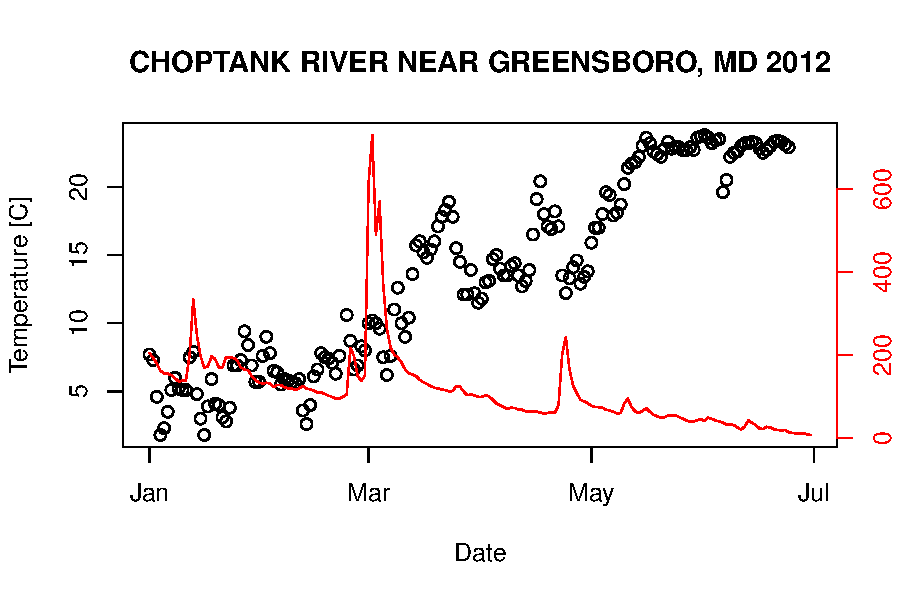
\includegraphics{dataRetrieval-fig1}
\end{center}
\caption{Temperature and discharge plot of Choptank River in 2012.}
\end{figure}


There are occasions where NWIS values are not reported as numbers, instead there might be text describing a certain event such as "Ice".  Any value that cannot be converted to a number will be reported as NA in this package.




%------------------------------------------------------------
\subsection{USGS Unit Value Retrievals}
%------------------------------------------------------------
We can also get real-time, instantaneous measurements using the retrieveUnitNWISData function:
\begin{Schunk}
\begin{Sinput}
> # Using defaults:
> siteNumber <- "01491000" # Site ID for Choptank River near Greensboro, MD
> parameterCd <- "00060"  # Discharge in cubic feet per second
> startDate <- as.character(Sys.Date()-1) # Yesterday 
>   # (or, the day before the dataRetrieval package was built)
> endDate <- as.character(Sys.Date()) # Today 
>   # (or, the day the dataRetrieval package was built)
> 
> dischargeToday <- retrieveUnitNWISData(siteNumber, parameterCd, startDate, endDate)
\end{Sinput}
\end{Schunk}
Which produces the following dataframe:
\begin{Schunk}
\begin{Soutput}
  agency_cd  site_no            datetime tz_cd X02_00060 X02_00060_cd
1      USGS 01491000 2013-01-23 00:00:00   EST       190            P
2      USGS 01491000 2013-01-23 00:15:00   EST       187            P
3      USGS 01491000 2013-01-23 00:30:00   EST       187            P
4      USGS 01491000 2013-01-23 00:45:00   EST       187            P
5      USGS 01491000 2013-01-23 01:00:00   EST       192            P
6      USGS 01491000 2013-01-23 01:15:00   EST       187            P
\end{Soutput}
\end{Schunk}
The structure of the dataframe is can be seen in Appendix 2: retrieveUnitNWISData. Note that time now becomes important, so the variable datetime is a POSIXct, and the time zone is included in a separate column. Data is pulled from \url{http://waterservices.usgs.gov/rest/IV-Test-Tool.html}. There are occasions where NWIS values are not reported as numbers, instead a common example is "Ice".  Any value that cannot be converted to a number will be reported as NA in this package.

A simple plotting example is shown in Figure 2:
\begin{Schunk}
\begin{Sinput}
> with(dischargeToday, plot(
   datetime, X02_00060,
   xlab="Date/Time",ylab="Discharge [cfs]"
   ))
\end{Sinput}
\end{Schunk}
\newpage

\begin{figure}
\begin{center}
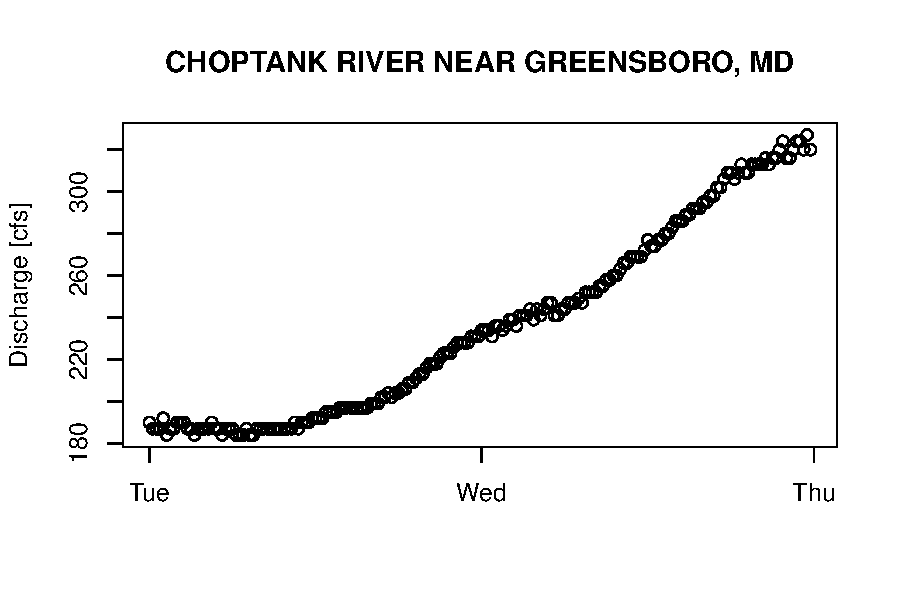
\includegraphics{dataRetrieval-fig2}
\end{center}
\caption{Real-time discharge plot of Choptank River.}
\end{figure}


%------------------------------------------------------------
\subsection{USGS Water Quality Retrievals}
%------------------------------------------------------------
Finally, we can use the dataRetrieval package to get water quality data that is available on the water quality data portal: \url{http://www.waterqualitydata.us/}. The raw data us obtained from the function  getRawQWData, with the similar input arguments: siteNumber, parameterCd, startDate, endDate, and interactive. The difference is in parameterCd, in this function multiple parameters can be queried using a ";" separator, and setting parameterCd <- "" will return all of the measured observations. The raw data can be overwelming (as will be demonstrated), a simplified version of the data can be obtained using getQWData.


\begin{Schunk}
\begin{Sinput}
> # Using defaults:
> siteNumber <- "01491000" # Site ID for Choptank River
> # Dissolved Nitrate parameter codes (one as mg/l as N, one as mg/l):
> parameterCd <- "00618;71851"  
> startDate <- "1964-06-11"
> endDate <- "2012-12-18"
> dissolvedNitrate <- getRawQWData(siteNumber, parameterCd, startDate, endDate)
\end{Sinput}
\end{Schunk}

There is a large amount of data returned for each observation. The available data can be viewed in Appendix 2: getRawQWData. To get a simplified dataframe that contains only datetime, value, and qualifier, use the function getQWData:

\begin{Schunk}
\begin{Sinput}
> dissolvedNitrateSimple <- getQWData(siteNumber, parameterCd, startDate, endDate)
> head(dissolvedNitrateSimple)
\end{Sinput}
\begin{Soutput}
     dateTime qualifier.71851 value.71851 qualifier.00618 value.00618
1  1964-06-11                         3.3                       0.745
3  1964-09-10                         5.3                       1.200
5  1965-02-01                         2.9                       0.655
7  1965-02-25                         2.4                       0.542
9  1965-03-25                         1.5                       0.339
11 1965-04-20                         2.2                       0.497
\end{Soutput}
\end{Schunk}
Note that in this dataframe, datatime is only imported as Dates (no times are included), and the qualifier is either blank or "<" signifying a censored value.

An example of plotting the above data (Figure 3):

\begin{Schunk}
\begin{Sinput}
> with(dissolvedNitrateSimple, plot(
   dateTime, value.00618,
   xlab="Date",ylab = paste(parameterINFO$srsname, "[",parameterINFO$parameter_units,"]")
   ))
\end{Sinput}
\end{Schunk}
\newpage

\begin{figure}
\begin{center}
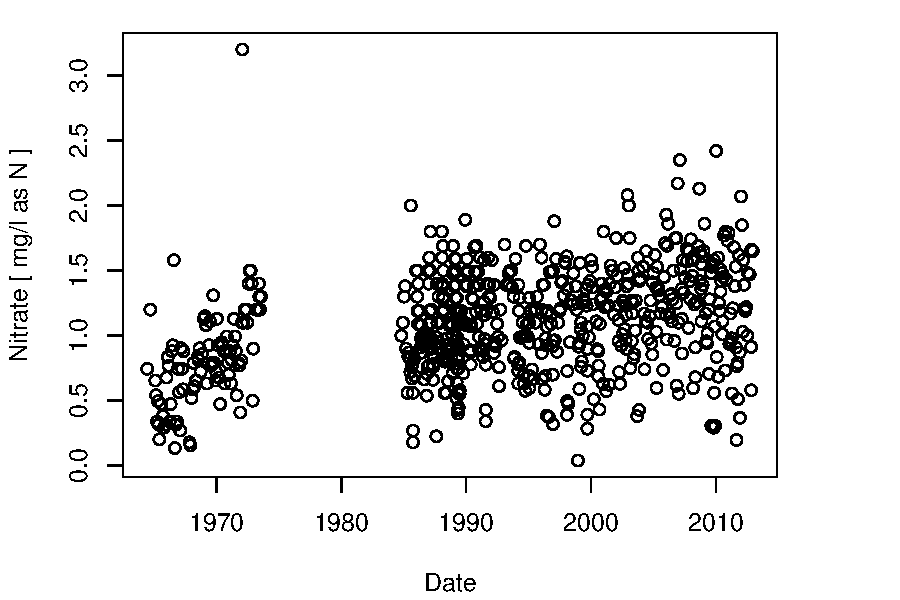
\includegraphics{dataRetrieval-fig3}
\end{center}
\caption{Nitrate plot of Choptank River.}
\end{figure}



%------------------------------------------------------------
\section{Polished Data: USGS Web Retrieval Examples}
%------------------------------------------------------------ 
Rather than using raw data as retrieved by the web, the dataRetrieval package also includes functions that return the data in a structure that has been designed to work with the EGRET R package (\url{https://github.com/USGS-R/EGRET/wiki}). In general, these dataframes may be much more 'R-friendly' than the raw data, and will contain additional information that allows for efficient data analysis.

In this section, we use 3 dataRetrieval functions to get sufficient data to perform an EGRET analysis.  We will continue analyzing the Choptank River. We will need essentially the same data that was retrieved in the previous section, but we will get the daily discharge values in a dataframe called Daily, the nitrate sample data in a dataframe called Sample, and the data about the station and parameters in a dataframe called INFO. These are the dataframes that were exclusively designed to work with the EGRET R package, however can be very useful for all hydrologic studies.

The funtion to obtain the daily values (discharge in this case) is getDVData.  It requires the inputs siteNumber, ParameterCd, StartDate, EndDate, interactive, and convert. Most of these arguments are described in the previous section, however 'convert' is a new argument, it's default is TRUE, and it tells the program to convert the values from cfs to cms. If you don't want this conversion, set convert=FALSE in the function call.

The function to obtain sample data from the water quality portal is getSampleData. The arguments for this function are also siteNumber, ParameterCd, StartDate, EndDate, interactive. These are the same inputs as getRawQWData or getQWData as described in the previous section.

The function to obtain "metadata", data about the gage station and measured parameters is getMetaData. This function essentially combines getSiteFileData and getParameterInfo, producing one dataframe called INFO.

The structure of each dataframe can be seen in Appendix 2.


\begin{Schunk}
\begin{Sinput}
> siteNumber <- "01491000" # Site ID for Choptank River near Greensboro, MD
> parameterCd <- "00631"  # Nitrate
> startDate <- "1964-01-01"
> endDate <- "2013-01-01"
> Daily <- getDVData(siteNumber, "00060", startDate, endDate)
\end{Sinput}
\begin{Soutput}
There are  17899 data points, and  17899 days.
There are  0 zero flow days
If there are any zero discharge days, all days had 0 cubic meters per second added to the discharge value.
\end{Soutput}
\begin{Sinput}
> Sample <-getSampleData(siteNumber,parameterCd,startDate, endDate)
> INFO <-getMetaData(siteNumber,parameterCd, interactive=FALSE)
> Sample <- mergeReport()
\end{Sinput}
\begin{Soutput}
 Discharge Record is 17899 days long, which is 49 years
 First day of the discharge record is 1964-01-01 and last day is 2013-01-01
 The water quality record has 627 samples
 The first sample is from 1973-06-04 and the last sample is from 2012-12-18
 Discharge: Minimum, mean and maximum 0.00991 4.02 246
 Concentration: Minimum, mean and maximum 0.05 1.1 2.4
 Percentage of the sample values that are censored is 0.16 %
\end{Soutput}
\begin{Sinput}
> head(Sample)
\end{Sinput}
\begin{Soutput}
        Date ConcLow ConcHigh Uncen ConcAve Julian Month Day  DecYear MonthSeq
1 1973-06-04    1.30     1.30     1    1.30  45079     6 155 1973.422     1482
2 1979-09-25    0.52     0.52     1    0.52  47383     9 268 1979.731     1557
3 1979-10-24    0.62     0.62     1    0.62  47412    10 297 1979.810     1558
4 1979-12-05    1.40     1.40     1    1.40  47454    12 339 1979.925     1560
5 1979-12-21    1.20     1.20     1    1.20  47470    12 355 1979.969     1560
6 1980-01-24    0.84     0.84     1    0.84  47504     1  24 1980.064     1561
       SinDY      CosDY         Q     LogQ
1  0.4699767 -0.8826788  3.256437 1.180634
2 -0.9927882 -0.1198812  3.398022 1.223193
3 -0.9295235  0.3687629  3.199804 1.163089
4 -0.4547551  0.8906165  2.973269 1.089662
5 -0.1961425  0.9805754  2.944952 1.080093
6  0.3925740  0.9197204 10.901986 2.388945
\end{Soutput}
\end{Schunk}

\newpage
%------------------------------------------------------------ 
\section{Appendix 1: Getting Started}
%------------------------------------------------------------ 
This section describes the options for downloading and installing the dataRetrieval package.

%------------------------------------------------------------
\subsection{New to R?}
%------------------------------------------------------------ 
If you are new to R, you will need to first install the latest version of R, which can be found here: \url{http://www.r-project.org/}.

There are many options for running and editing R code, one nice enviornment to learn R is RStudio. RStudio can be downloaded here: \url{http://rstudio.org/}. Once R and RStudio are installed, the dataRetrieval package needs to be installed as described in the next section.

%------------------------------------------------------------
\subsection{R User: Installing dataRetrieval from downloaded binary}
%------------------------------------------------------------ 
The latest dataRetrieval package build is available for download at \url{https://github.com/USGS-R/dataRetrieval/blob/master/dataRetrieval_1.2.1.tar.gz}.  If the package's tar.gz file is saved in R's working directory, then the following command will fully install the package:

\begin{Schunk}
\begin{Sinput}
> install.packages("dataRetrieval_1.2.1.tar.gz", 
                  repos=NULL, type="source")
\end{Sinput}
\end{Schunk}

If the downloaded file is stored in an alternative location, include the path in the install command.  A Windows example looks like this (notice the direction of the slashes, they are in the opposite direction that Windows normally creates paths):

\begin{Schunk}
\begin{Sinput}
> install.packages(
   "C:/RPackages/Statistics/dataRetrieval_1.2.1.tar.gz", 
   repos=NULL, type="source")
\end{Sinput}
\end{Schunk}

A Mac example looks like this:

\begin{Schunk}
\begin{Sinput}
> install.packages(
   "/Users/userA/RPackages/Statistic/dataRetrieval_1.2.1.tar.gz", 
   repos=NULL, type="source")
\end{Sinput}
\end{Schunk}

It is a good idea to re-start the R enviornment after installing the package, especially if installing an updated version (that is, restart RStudio). Some users have found it necessary to delete the previous version's package folder before installing newer version of dataRetrieval. If you are experiencing issues after updating a package, trying deleting the package folder - the default location for Windows is something like this: C:/Users/userA/Documents/R/win-library/2.15/dataRetrieval, and the default for a Mac: /Users/userA/Library/R/2.15/library/dataRetrieval. Then, re-install the package using the directions above. Moving to CRAN should solve this problem.

After installing the package, you need to open the library each time you re-start R.  This is done with the simple command:
\begin{Schunk}
\begin{Sinput}
> library(dataRetrieval)
\end{Sinput}
\end{Schunk}
Using RStudio, you could alternatively click on the checkbox for dataRetrieval in the Packages window.

%------------------------------------------------------------
\subsection{R Developers: Installing dataRetrieval from gitHub}
%------------------------------------------------------------
Alternatively, R-developers can install the latest version of dataRetrieval directly from gitHub using the devtools package.  devtools is available on CRAN.  Simpley type the following commands into R to install the latest version of dataRetrieval available on gitHub.  Rtools (for Windows) and appropriate \LaTeX\ tools are required.

\begin{Schunk}
\begin{Sinput}
> library(devtools)
> install_github("dataRetrieval", "USGS-R")
\end{Sinput}
\end{Schunk}
To then open the library, simply type:

\begin{Schunk}
\begin{Sinput}
> library(dataRetrieval)
\end{Sinput}
\end{Schunk}

\newpage
%------------------------------------------------------------ 
\section{Appendix 2: Dataframe column names and data types}
%------------------------------------------------------------ 
This section shows the returned dataframe structures for the functions.  The requested data is the same as in earlier sections of this document:
\begin{Schunk}
\begin{Sinput}
> library(dataRetrieval)
> siteNumber <- "01491000" # Site ID for Choptank River near Greensboro, MD
> parameterCd <- "00631"  # Nitrate
> startDate <- "1964-01-01"
> endDate <- "2013-01-01"
> 
\end{Sinput}
\end{Schunk}

%------------------------------------------------------------
\subsection{getSiteFileData}
%------------------------------------------------------------
\begin{Schunk}
\begin{Sinput}
> ChoptankInfo <- getSiteFileData(siteNumber)
\end{Sinput}
\end{Schunk}
\begin{Schunk}
\begin{Sinput}
> str(ChoptankInfo)
\end{Sinput}
\begin{Soutput}
'data.frame':	1 obs. of  43 variables:
 $ agency.cd            : chr "USGS"
 $ site.no              : chr "01491000"
 $ station.nm           : chr "CHOPTANK RIVER NEAR GREENSBORO, MD"
 $ site.tp.cd           : chr "ST"
 $ lat.va               : chr "385949.9"
 $ long.va              : chr "0754708.9"
 $ dec.lat.va           : num 39
 $ dec.long.va          : num -75.8
 $ coord.meth.cd        : chr "M"
 $ coord.acy.cd         : chr "S"
 $ coord.datum.cd       : chr "NAD83"
 $ dec.coord.datum.cd   : chr "NAD83"
 $ district.cd          : chr "24"
 $ state.cd             : chr "24"
 $ county.cd            : chr "011"
 $ country.cd           : chr "US"
 $ land.net.ds          : chr ""
 $ map.nm               : chr ""
 $ map.scale.fc         : chr ""
 $ alt.va               : num 3.51
 $ alt.meth.cd          : chr "L"
 $ alt.acy.va           : chr ".01"
 $ alt.datum.cd         : chr "NGVD29"
 $ huc.cd               : chr "02060005"
 $ basin.cd             : chr ""
 $ topo.cd              : chr ""
 $ instruments.cd       : chr "YYNNYNYNNNYNNNNNNNNNNNNNNNNNNN"
 $ construction.dt      : chr ""
 $ inventory.dt         : chr ""
 $ drain.area.va        : chr "113"
 $ contrib.drain.area.va: chr ""
 $ tz.cd                : chr "EST"
 $ local.time.fg        : chr "N"
 $ reliability.cd       : chr ""
 $ gw.file.cd           : chr "NNNNNNNN"
 $ nat.aqfr.cd          : chr ""
 $ aqfr.cd              : chr ""
 $ aqfr.type.cd         : chr ""
 $ well.depth.va        : chr ""
 $ hole.depth.va        : chr ""
 $ depth.src.cd         : chr ""
 $ project.no           : chr "442400300"
 $ queryTime            : POSIXct, format: "2013-01-24 10:35:51"
\end{Soutput}
\end{Schunk}


%------------------------------------------------------------
\subsection{getParameterInfo}
%------------------------------------------------------------
\begin{Schunk}
\begin{Sinput}
> parameterINFO <- getParameterInfo(parameterCd, interactive=FALSE)
> str(parameterINFO)
\end{Sinput}
\begin{Soutput}
'data.frame':	1 obs. of  6 variables:
 $ parameter_cd      : chr "00631"
 $ parameter_group_nm: chr "Nutrient"
 $ parameter_nm      : chr "Nitrate plus nitrite, water, filtered, milligrams per liter as nitrogen"
 $ casrn             : chr ""
 $ srsname           : chr "Inorganic nitrogen (nitrate and nitrite)"
 $ parameter_units   : chr "mg/l as N"
\end{Soutput}
\end{Schunk}

%------------------------------------------------------------
\subsection{getMetaData}
%------------------------------------------------------------
\begin{Schunk}
\begin{Sinput}
> INFO <- getMetaData(siteNumber,parameterCd, interactive=FALSE)
> str(INFO)
\end{Sinput}
\begin{Soutput}
'data.frame':	1 obs. of  41 variables:
 $ agency.cd            : chr "USGS"
 $ site.no              : chr "01491000"
 $ station.nm           : chr "CHOPTANK RIVER NEAR GREENSBORO, MD"
 $ site.tp.cd           : chr "ST"
 $ lat.va               : chr "385949.9"
 $ long.va              : chr "0754708.9"
 $ dec.lat.va           : num 39
 $ dec.long.va          : num -75.8
 $ coord.meth.cd        : chr "M"
 $ coord.acy.cd         : chr "S"
 $ coord.datum.cd       : chr "NAD83"
 $ dec.coord.datum.cd   : chr "NAD83"
 $ district.cd          : chr "24"
 $ state.cd             : chr "24"
 $ county.cd            : chr "011"
 $ country.cd           : chr "US"
 $ map.nm               : chr ""
 $ map.scale.fc         : chr ""
 $ alt.va               : num 3.51
 $ alt.meth.cd          : chr "L"
 $ alt.acy.va           : chr ".01"
 $ alt.datum.cd         : chr "NGVD29"
 $ huc.cd               : chr "02060005"
 $ basin.cd             : chr ""
 $ topo.cd              : chr ""
 $ construction.dt      : chr ""
 $ inventory.dt         : chr ""
 $ drain.area.va        : num 113
 $ contrib.drain.area.va: num NA
 $ tz.cd                : chr "EST"
 $ local.time.fg        : chr "N"
 $ reliability.cd       : chr ""
 $ project.no           : chr "442400300"
 $ queryTime            : POSIXct, format: "2013-01-24 10:36:02"
 $ drainSqKm            : num 293
 $ staAbbrev            : logi NA
 $ param.nm             : chr "Nitrate plus nitrite, water, filtered, milligrams per liter as nitrogen"
 $ param.units          : chr "mg/l as N"
 $ paramShortName       : chr "Inorganic nitrogen (nitrate and nitrite)"
 $ paramNumber          : chr "00631"
 $ constitAbbrev        : chr "Inorganic nitrogen (nitrate and nitrite)"
\end{Soutput}
\end{Schunk}

%------------------------------------------------------------
\subsection{retrieveNWISData}
%------------------------------------------------------------
\begin{Schunk}
\begin{Sinput}
> parameterCd <- "00010,00060"  # Temperature and discharge
> statCd <- "00001,00003"  #mean and maximum
> startDate <- "2012-01-01"
> endDate <- "2012-06-30"
> temperatureAndFlow <- retrieveNWISData(siteNumber, parameterCd, 
        startDate, endDate, StatCd=statCd,interactive=FALSE)
> str(temperatureAndFlow)
\end{Sinput}
\begin{Soutput}
'data.frame':	182 obs. of  9 variables:
 $ agency_cd         : chr  "USGS" "USGS" "USGS" "USGS" ...
 $ site_no           : chr  "01491000" "01491000" "01491000" "01491000" ...
 $ datetime          : Date, format: "2012-01-01" "2012-01-02" ...
 $ X01_00010_00001   : num  8.4 8.5 6 3 2.9 4.7 5.9 6.3 5.9 5.5 ...
 $ X01_00010_00001_cd: chr  "P" "P" "P" "P" ...
 $ X01_00010_00003   : num  7.7 7.3 4.6 1.8 2.3 3.5 5.1 6 5.2 5.1 ...
 $ X01_00010_00003_cd: chr  "P" "P" "P" "P" ...
 $ X02_00060_00003   : num  205 193 180 162 155 155 151 144 136 138 ...
 $ X02_00060_00003_cd: chr  "A" "A" "A" "A" ...
\end{Soutput}
\end{Schunk}

%------------------------------------------------------------
\subsection{retrieveUnitNWISData}
%------------------------------------------------------------
\begin{Schunk}
\begin{Sinput}
> parameterCd <- "00060"  # Discharge in cubic feet per second
> startDate <- as.character(Sys.Date()-1) # Yesterday 
>   # (or, the day before the dataRetrieval package was built)
> endDate <- as.character(Sys.Date()) # Today 
>   # (or, the day the dataRetrieval package was built)
> 
> dischargeToday <- retrieveUnitNWISData(siteNumber, parameterCd, startDate, endDate)
> str(dischargeToday)
\end{Sinput}
\begin{Soutput}
'data.frame':	142 obs. of  6 variables:
 $ agency_cd   : chr  "USGS" "USGS" "USGS" "USGS" ...
 $ site_no     : chr  "01491000" "01491000" "01491000" "01491000" ...
 $ datetime    : POSIXct, format: "2013-01-23 00:00:00" "2013-01-23 00:15:00" ...
 $ tz_cd       : chr  "EST" "EST" "EST" "EST" ...
 $ X02_00060   : num  190 187 187 187 192 187 192 187 187 187 ...
 $ X02_00060_cd: chr  "P" "P" "P" "P" ...
\end{Soutput}
\end{Schunk}

%------------------------------------------------------------
\subsection{getDVData}
%------------------------------------------------------------
\begin{Schunk}
\begin{Sinput}
> startDate <- "1964-01-01"
> endDate <- "2013-01-01"
> Daily <- getDVData(siteNumber, "00060", startDate, endDate)
\end{Sinput}
\begin{Soutput}
There are  17899 data points, and  17899 days.
There are  0 zero flow days
If there are any zero discharge days, all days had 0 cubic meters per second added to the discharge value.
\end{Soutput}
\begin{Sinput}
> str(Daily)
\end{Sinput}
\begin{Soutput}
'data.frame':	17899 obs. of  12 variables:
 $ Date     : Date, format: "1964-01-01" "1964-01-02" ...
 $ Q        : num  1.67 5.47 7.11 4.47 2.52 ...
 $ Julian   : num  41637 41638 41639 41640 41641 ...
 $ Month    : num  1 1 1 1 1 1 1 1 1 1 ...
 $ Day      : num  1 2 3 4 5 6 7 8 9 10 ...
 $ DecYear  : num  1964 1964 1964 1964 1964 ...
 $ MonthSeq : num  1369 1369 1369 1369 1369 ...
 $ Qualifier: chr  "A" "A" "A" "A" ...
 $ i        : int  1 2 3 4 5 6 7 8 9 10 ...
 $ LogQ     : num  0.513 1.698 1.961 1.498 0.924 ...
 $ Q7       : num  NA NA NA NA NA ...
 $ Q30      : num  NA NA NA NA NA NA NA NA NA NA ...
\end{Soutput}
\end{Schunk}

%------------------------------------------------------------
\subsection{getRawQWData}
%------------------------------------------------------------
\begin{Schunk}
\begin{Sinput}
> parameterCd <- "00618;71851"  
> dissolvedNitrate <- getRawQWData(siteNumber, parameterCd, startDate, endDate)
> str(dissolvedNitrate)
\end{Sinput}
\begin{Soutput}
'data.frame':	1402 obs. of  62 variables:
 $ OrganizationIdentifier                           : chr  "USGS-MD" "USGS-MD" "USGS-MD" "USGS-MD" ...
 $ OrganizationFormalName                           : chr  "USGS Maryland Water Science Center" "USGS Maryland Water Science Center" "USGS Maryland Water Science Center" "USGS Maryland Water Science Center" ...
 $ ActivityIdentifier                               : chr  "nwismd.01.96400030" "nwismd.01.96400030" "nwismd.01.96400031" "nwismd.01.96400031" ...
 $ ActivityTypeCode                                 : chr  "Sample-Routine" "Sample-Routine" "Sample-Routine" "Sample-Routine" ...
 $ ActivityMediaName                                : chr  "Water" "Water" "Water" "Water" ...
 $ ActivityMediaSubdivisionName                     : chr  "Surface Water" "Surface Water" "Surface Water" "Surface Water" ...
 $ ActivityStartDate                                : chr  "1964-06-11" "1964-06-11" "1964-09-10" "1964-09-10" ...
 $ ActivityStartTime.Time                           : chr  "" "" "" "" ...
 $ ActivityStartTime.TimeZoneCode                   : chr  "" "" "" "" ...
 $ ActivityEndDate                                  : chr  "" "" "" "" ...
 $ ActivityEndTime.Time                             : chr  "" "" "" "" ...
 $ ActivityEndTime.TimeZoneCode                     : chr  "" "" "" "" ...
 $ ActivityDepthHeightMeasure.MeasureValue          : chr  "" "" "" "" ...
 $ ActivityDepthHeightMeasure.MeasureUnitCode       : chr  "" "" "" "" ...
 $ ActivityDepthAltitudeReferencePointText          : chr  "" "" "" "" ...
 $ ActivityTopDepthHeightMeasure.MeasureValue       : chr  "" "" "" "" ...
 $ ActivityTopDepthHeightMeasure.MeasureUnitCode    : chr  "" "" "" "" ...
 $ ActivityBottomDepthHeightMeasure.MeasureValue    : chr  "" "" "" "" ...
 $ ActivityBottomDepthHeightMeasure.MeasureUnitCode : chr  "" "" "" "" ...
 $ ProjectIdentifier                                : chr  "USGS" "USGS" "USGS" "USGS" ...
 $ ActivityConductingOrganizationText               : chr  "" "" "" "" ...
 $ MonitoringLocationIdentifier                     : chr  "USGS-01491000" "USGS-01491000" "USGS-01491000" "USGS-01491000" ...
 $ ActivityCommentText                              : chr  "" "" "" "" ...
 $ SampleAquifer                                    : chr  "" "" "" "" ...
 $ HydrologicCondition                              : chr  "Not determined" "Not determined" "Not determined" "Not determined" ...
 $ HydrologicEvent                                  : chr  "Routine sample" "Routine sample" "Routine sample" "Routine sample" ...
 $ SampleCollectionMethod.MethodIdentifier          : chr  "USGS" "USGS" "USGS" "USGS" ...
 $ SampleCollectionMethod.MethodIdentifierContext   : chr  "USGS" "USGS" "USGS" "USGS" ...
 $ SampleCollectionMethod.MethodName                : chr  "USGS" "USGS" "USGS" "USGS" ...
 $ SampleCollectionEquipmentName                    : chr  "Unknown" "Unknown" "Unknown" "Unknown" ...
 $ ResultDetectionConditionText                     : chr  "" "" "" "" ...
 $ CharacteristicName                               : chr  "Nitrate" "Nitrate" "Nitrate" "Nitrate" ...
 $ ResultSampleFractionText                         : chr  "Dissolved" "Dissolved" "Dissolved" "Dissolved" ...
 $ ResultMeasureValue                               : chr  "3.30" "0.745" "5.30" "1.20" ...
 $ ResultMeasure.MeasureUnitCode                    : chr  "mg/l" "mg/l as N" "mg/l" "mg/l as N" ...
 $ MeasureQualifierCode                             : chr  "" "" "" "" ...
 $ ResultStatusIdentifier                           : chr  "Historical" "Historical" "Historical" "Historical" ...
 $ StatisticalBaseCode                              : chr  "" "" "" "" ...
 $ ResultValueTypeName                              : chr  "Actual" "Calculated" "Actual" "Calculated" ...
 $ ResultWeightBasisText                            : chr  "" "" "" "" ...
 $ ResultTimeBasisText                              : chr  "" "" "" "" ...
 $ ResultTemperatureBasisText                       : chr  "" "" "" "" ...
 $ ResultParticleSizeBasisText                      : chr  "" "" "" "" ...
 $ PrecisionValue                                   : chr  "" "" "" "" ...
 $ ResultCommentText                                : chr  "" "" "" "" ...
 $ USGSPCode                                        : chr  "71851" "00618" "71851" "00618" ...
 $ ResultDepthHeightMeasure.MeasureValue            : chr  "" "" "" "" ...
 $ ResultDepthHeightMeasure.MeasureUnitCode         : chr  "" "" "" "" ...
 $ ResultDepthAltitudeReferencePointText            : chr  "" "" "" "" ...
 $ SubjectTaxonomicName                             : chr  "" "" "" "" ...
 $ SampleTissueAnatomyName                          : chr  "" "" "" "" ...
 $ ResultAnalyticalMethod.MethodIdentifier          : chr  "" "ALGOR" "" "ALGOR" ...
 $ ResultAnalyticalMethod.MethodIdentifierContext   : chr  "" "USGS" "" "USGS" ...
 $ ResultAnalyticalMethod.MethodName                : chr  "" "Computation by NWIS algorithm" "" "Computation by NWIS algorithm" ...
 $ MethodDescriptionText                            : chr  "" "NWIS User's Manual, QW System, Appendix" "" "NWIS User's Manual, QW System, Appendix" ...
 $ LaboratoryName                                   : chr  "" "" "" "" ...
 $ AnalysisStartDate                                : chr  "" "" "" "" ...
 $ ResultLaboratoryCommentText                      : chr  "" "" "" "" ...
 $ DetectionQuantitationLimitTypeName               : chr  "" "" "" "" ...
 $ DetectionQuantitationLimitMeasure.MeasureValue   : chr  "" "" "" "" ...
 $ DetectionQuantitationLimitMeasure.MeasureUnitCode: chr  "" "" "" "" ...
 $ PreparationStartDate                             : chr  "" "" "" "" ...
\end{Soutput}
\end{Schunk}

%------------------------------------------------------------
\subsection{getQWData}
%------------------------------------------------------------
\begin{Schunk}
\begin{Sinput}
> dissolvedNitrateSimple <- getQWData(siteNumber, parameterCd, startDate, endDate)
> str(dissolvedNitrateSimple)
\end{Sinput}
\begin{Soutput}
'data.frame':	657 obs. of  5 variables:
 $ dateTime       : Date, format: "1964-06-11" "1964-09-10" ...
 $ qualifier.71851: chr  "" "" "" "" ...
 $ value.71851    : num  3.3 5.3 2.9 2.4 1.5 2.2 1.4 0.9 2.1 1.7 ...
 $ qualifier.00618: chr  "" "" "" "" ...
 $ value.00618    : num  0.745 1.2 0.655 0.542 0.339 0.497 0.316 0.203 0.474 0.384 ...
 - attr(*, "reshapeWide")=List of 5
  ..$ v.names: NULL
  ..$ timevar: chr "USGSPCode"
  ..$ idvar  : chr "dateTime"
  ..$ times  : Factor w/ 2 levels "00618","71851": 2 1
  ..$ varying: chr [1:2, 1:2] "qualifier.71851" "value.71851" "qualifier.00618" "value.00618"
\end{Soutput}
\end{Schunk}

%------------------------------------------------------------
\subsection{getSampleData}
%------------------------------------------------------------
\begin{Schunk}
\begin{Sinput}
> Sample <-getSampleData(siteNumber,parameterCd,startDate, endDate)
> str(Sample)
\end{Sinput}
\begin{Soutput}
'data.frame':	657 obs. of  12 variables:
 $ Date    : Date, format: "1964-06-11" "1964-09-10" ...
 $ ConcLow : num  4.04 6.5 3.55 2.94 1.84 ...
 $ ConcHigh: num  4.04 6.5 3.55 2.94 1.84 ...
 $ Uncen   : num  1 1 1 1 1 1 1 1 1 1 ...
 $ ConcAve : num  4.04 6.5 3.55 2.94 1.84 ...
 $ Julian  : num  41799 41890 42034 42058 42086 ...
 $ Month   : num  6 9 2 2 3 4 5 6 7 9 ...
 $ Day     : num  163 254 32 56 84 110 134 152 207 257 ...
 $ DecYear : num  1964 1965 1965 1965 1965 ...
 $ MonthSeq: num  1374 1377 1382 1382 1383 ...
 $ SinDY   : num  0.345 -0.936 0.515 0.815 0.991 ...
 $ CosDY   : num  -0.939 -0.353 0.857 0.579 0.137 ...
\end{Soutput}
\end{Schunk}


%------------------------------------------------------------
% BIBLIO
%------------------------------------------------------------
\begin{thebibliography}{10}

\bibitem{HirschI}
Helsel, D.R. and R. M. Hirsch, 2002. Statistical Methods in Water Resources Techniques of Water Resources Investigations, Book 4, chapter A3. U.S. Geological Survey. 522 pages. \url{http://pubs.usgs.gov/twri/twri4a3/}

\bibitem{HirschII}
Hirsch, R. M., Moyer, D. L. and Archfield, S. A. (2010), Weighted Regressions on Time, Discharge, and Season (WRTDS), with an Application to Chesapeake Bay River Inputs. JAWRA Journal of the American Water Resources Association, 46: 857-880. doi: 10.1111/j.1752-1688.2010.00482.x \url{http://onlinelibrary.wiley.com/doi/10.1111/j.1752-1688.2010.00482.x/full}

\bibitem{HirschIII}
Sprague, L. A., Hirsch, R. M., and Aulenbach, B. T. (2011), Nitrate in the Mississippi River and Its Tributaries, 1980 to 2008: Are We Making Progress? Environmental Science \& Technology, 45 (17): 7209-7216. doi: 10.1021/es201221s \url{http://pubs.acs.org/doi/abs/10.1021/es201221s}

\end{thebibliography}

\end{document}

\end{document}
